\documentclass{article}

\usepackage[vmarginratio=1:1,a4paper,body={6.5in, 9.5in}]{geometry}

\usepackage[T2A]{fontenc}
\usepackage[utf8]{inputenc}
\usepackage[russian]{babel}

\usepackage{amsmath}
\usepackage{amssymb}
\usepackage{amsfonts}
\usepackage{amsthm}
\usepackage{color}

\usepackage{hyperref}
\usepackage{graphicx}

\usepackage{mathtools}
\DeclarePairedDelimiter{\diagfences}{(}{)}
\newcommand{\diag}{\operatorname{diag}\diagfences}


\title{Reaction wheel 1D pendulum}
\author{}
\date{}

\begin{document}

\maketitle
% The Reaction Wheel Pendulum (Block, Atrom, Spong)
%ftp://nozdr.ru/biblio/kolxo3/P/PC/PCtm/Block%20D.,%20Astroem%20K.,%20Spong%20M.%20The%20Reaction%20Wheel%20Pendulum%20(MC,%202007)(ISBN%201598291947)(O)(112s)_PCtm_.pdf

\section{Вывод уравнений движения}

\begin{minipage}[t]{.2\linewidth}
\vspace{0cm}
\centerline{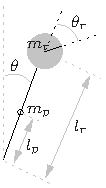
\includegraphics[width=\linewidth]{img/schema}}
\end{minipage}
\begin{minipage}[t]{.8\linewidth}
\vspace{0cm}
\begin{itemize}
    \item $m_p$ - масса маятника
    \item $m_r$ - масса ротора
    \item $l_p$ - расстояние от шарнира до центра масс маятника
    \item $l_r$ - расстояние от шарнира до центра масс ротора
    \item $J_p$ - момент инерции маятника при вращении вокруг центра масс
    \item $J_r$ - момент инерции ротора
    \item $\theta$ - угол маятника относительно вертикали
    \item $\theta_r$ - угол ротора \textbf{относительно маятника}
    \item $\tau$ - момент, прикладываемый к ротору
    \item $C_p$ - коэффициент вязкого трения в шарнире маятника
    \item $C_r$ - коэффициент вязкого трения ротора
\end{itemize}
\end{minipage}

\vspace{5mm}

Кинетическая энергия маятника:
$$
T_p = \frac{1}{2} (m_pl_p^2 + J_p)\dot\theta^2
$$

Кинетическая энергия маховика:
$$
T_r = \frac{1}{2} m_r l_r^2 \dot\theta^2 + \frac{1}{2}J_r (\dot\theta_r+\dot\theta)^2
$$

Общая потенциальная энергия:
$$
P = (m_pl_p + m_r l_r)g \cos\theta
$$

Лагранжиан:
$$
\mathcal{L} = T_p + T_r - P
$$

Введём новые обозначения констант, которые нам уменьшат общее количество закорючек в уравнениях:
\begin{align*}
ml&:=m_p l_p + m_r l_r\\
J &:= J_p + m_p l_p^2 + m_r l_r^2
\end{align*}

Тогда лагранжиан запишется следующим образом:
$$
\mathcal L = \frac{1}{2}J\dot\theta^2 + \frac{1}{2}J_r(\dot\theta_r+\dot\theta)^2 - mlg\cos\theta
$$

Для удобства выпишем все частные производные:
\begin{align*}
\frac{\partial\mathcal L}{\partial\dot\theta_r} &= J_r(\dot\theta_r + \dot\theta)       & \frac{\partial\mathcal L}{\partial\theta_r} &= 0            \\
\frac{\partial\mathcal L}{\partial\dot\theta}   &= (J+J_r)\dot\theta + J_r\dot\theta_r  & \frac{\partial\mathcal L}{\partial\theta}   &= mlg\sin\theta\\
\end{align*}

Напоминалка про уравнения Лагранжа:
$$
\frac{d}{dt}\left(\frac{\partial\mathcal L}{\partial\dot q_i}\right) - \frac{\partial\mathcal L}{\partial q_i} = \tau_i
$$

Тогда уравнения движения примут следующий вид:
\begin{align*}
J_r\ddot\theta_r + J_r\ddot\theta&= - C_r \dot\theta_r + \tau\\
(J+J_r)\ddot \theta + J_r\ddot\theta_r - mlg\sin\theta &= - C_p \dot\theta 
\end{align*}

Перепишем, оставив вторые производные слева:
$$
\left\{
\begin{array}{l}
\ddot\theta_r = \frac{J+J_r}{J J_r}(\tau - C_r\dot\theta_r) - \frac{mlg}{J}\sin\theta + \frac{C_p}{J}\dot\theta\\
\ddot\theta   = -\frac{\tau}{J} + \frac{ml g}{J}\sin\theta  - \frac{C_p}{J} \dot\theta + \frac{C_r}{J} \dot\theta_r
\end{array}
\right.
$$



Наверняка трение в маятнике будет существенно ниже трения в роторе, и вполне возможно, что при этом пренебречь можно будет обоими. 


{\color{blue} Эти уравнения движения полностью совпадают с уравнениями из \href{https://www.ethz.ch/content/dam/ethz/special-interest/mavt/dynamic-systems-n-control/idsc-dam/Research_DAndrea/Cubli/Cubli_IROS2012.pdf}{The Cubli: A Cube that can Jump Up and Balance}, а также с уравнениями из \href{https://dl.acm.org/citation.cfm?id=3019246}{The Reaction Wheel Pendulum} (с точностью до выбора переменных, Åström отсчитывает угол ротора от вертикали). Но Åström в уравнения Лагранжа вставляет моменты $\tau$ и $-\tau$, а я тут вставляются $\tau$ и 0. Подход Острёма интуитивно понятен: если на ротор действует момент $\tau$, то на маятник действует момент $-\tau$. Впрочем, это зависит от выбора репера ($\theta_r$ отсчитывается от вертикали или от маятника). Нечего выбирать неортогональные базисы пространства конфигураций.}


\section{Как выбрать размер маховика?}

Здесь я напишу уравнения движения для обычного коллекторного двигателя, но для бесколлекторных уравнения примерно такие же.  Подадим на клеммы мотора максимально возможное напряжение, для заданного маховика задача состоит в том, чтобы найти максимально возможный угол начального отклонения маятника, при котором разгоняющийся маховик сможет перекинуть маятник через ноль. Затем будем варьировать размер маховика и смотреть, как будет изменяться максимально возможный угол отклонения.

Заглянем в даташит мотора:
\begin{itemize}
    \item $L$ - индуктивность обмотки
    \item $R$ - сопротивление обмотки
    \item $k$ - torque constant (= back-EMF constant)
\end{itemize}

Добавим в уравнения движения уравнение мотора:
$$
\left\{
\begin{array}{l}
\ddot\theta_r = \frac{J+J_r}{J J_r}(kI - C_r\dot\theta_r)  -mlg/J\sin\theta + C_p/J\dot\theta\\
\ddot \theta  = -k/J I + mlg/J\sin\theta - C_p/J \dot\theta + C_r/J \dot\theta_r\\
\dot I  = U/L - R/LI - k/L \dot\theta_r\\
\end{array}
\right.
$$

Для грубой прикидки размера маховика будем пренебрегать всяким. Индуктивность обмоток мотора очень низкая, поэтому можно сказать, что $I=U/R-K/R\,\dot\theta_r$. Вязкие трения тоже убираем, $C_r=C_P=0$. 
Рабочая зона наверняка будет узкой, поэтому заменим синус напрямую на его аргумент. Мысль такая: если будет стабилизироваться линеаризованная модель, то с синусом и подавно маятник встанет. Тогда уравнения движения будут выглядеть следующим образом:
$$
\left\{
\begin{array}{l}
\ddot\theta_r = \frac{J+J_r}{J J_r}(\frac{k\,U}{R} - \frac{k^2}{R}\dot\theta_r)  - \frac{mlg}{J}\theta\\
\ddot \theta  = -\frac{k\,U}{J\,R} + \frac{k^2}{J\,R}\dot\theta_r + \frac{mlg}{J}\theta
\end{array}
\right.
$$

Ну или в матричном виде: 
$$
\frac{d}{dt}\begin{pmatrix}\theta \\ \dot\theta \\ \dot\theta_r \end{pmatrix} = A \begin{pmatrix}\theta \\ \dot\theta \\ \dot\theta_r \end{pmatrix} + B U,
$$
где:
$$
A= \begin{pmatrix} 0 & 1 & 0 \\ \frac{mlg}{J} & 0 & \frac{k^2}{JR} \\ -\frac{mlg}{J} & 0 & -\frac{(J+J_r)k^2}{J\,J_r\,R} \end{pmatrix},
\qquad 
B=\begin{pmatrix}0\\ -\frac{k}{JR} \\ \frac{(J+J_r)k}{J\,J_r\,R} \end{pmatrix}.
$$

На всякий случай выпишем характеристический многочлен:
$$\chi(\lambda) = -\lambda^3 - \frac{k^2(J_r+J)}{JrJR}\,\lambda^2 + \frac{lmg}{J}\,\lambda+\frac{lmgk^2}{J_rJR}.$$
Он имеет три различных вещественных корня, два из них отрицательных, один положительный. В этом легко убедиться:
$$
\chi(0)>0,\quad \lim\limits_{\lambda\rightarrow-\infty}\chi(\lambda)=+\infty,\quad \lim\limits_{\lambda\rightarrow+\infty}\chi(\lambda)=-\infty,\quad\chi\left(-\sqrt{\frac{lmg}{J}}\right) = -\frac{lmg k^2}{J^2 R}<0.
$$
Аргумент в последнем неравенстве вылез из желания взаимоуничтожить кубическое и линейное слагаемые многочлена.
Положительное собственное число говорит о том, что в отсутствие управления система у нас неустойчива.
Поскольку у нас три различных вещественных корня, то матрица $A$ будет иметь полный набор вещественных собственных векторов, соответственно можно произвести её спектральное разложение $A = V \Lambda V^{-1}$, где $V$ - это матрица, составленная из трёх собственных векторов-столбцов, а $\Lambda=\diag{\lambda_1, \lambda_2, \lambda_3}$ - диагональная матрица собственных чисел.
Не умаляя общности, будем считать, что $\lambda_1>0>\lambda_2>\lambda_3$.

Наша задача найти зону устойчивости нашего диффура. Для начала сделаем замену переменной $x=Vy$.
Тогда наше уравнение $\dot x = Ax + BU$ перепишется как $V\dot y = AVy + BU$. Домножим слева на $V^{-1}$: 
$$
\dot y = V^{-1}AVy + V^{-1}BU = \Lambda y + V^{-1}BU.
$$
Эта замена переменной сделана для того, чтобы зона устойчивости имела красивое выражение, будучи разложенной на независимые переменные.
В силу диагональности новой матрицы системы, вторая и третья координата $y$ нас не интересуют вообще, нам интересна координата, которая соответствует положительному собственному числу.
Обозначим через $b_1$ первую координату вектора $V^{-1}BU$ (напоминаю, что у нас напряжение $U$ постоянно).
Вполне очевидно, что зона устойчивости этого диффура представляет собой пространство между двумя плоскостями $\left(-\frac{|b_1|}{\lambda_1}, \frac{|b_1|}{\lambda_1} \right) \times \mathbb R \times \mathbb R$.

Это прекрасно, но нас интересует устойчивость в терминах изначальных переменных.
Если мы сделаем обратное преобразование, то в пространстве $x$ зона устойчивости также будет заключена между двумя параллельными плоскостями.
Плоскости будут наклонными, т.к. мы себе можем позволить больший угол отклонения, если правильно подкрутить начальные скорости.
Но нас интересует конкретный случай, когда обе скорости нулевые. Самый простой способ это посчитать - это взять луч с направляющим вектором $(1,0,0)$, преобразовать его при помощи $V^{-1}$,
пересечь с плоскостью $y_1 = \frac{|b_1|}{\lambda_1}$, а затем точку пересечения обратно преобразовать при помощи $V$.

Решаем численно, так как очень уж громоздко выписывать собственные вектора символьно. Картинка~\ref{fig:rwdiameter} показывает максимальный угол, из которого можно стабилизировать маятник, для данного диаметра маховика.







%Решаем численно, перебираем значения обычными вложенными циклами. Зависимость максимального угла от радиуса маховика (алюминиевый цилиндр высоты 20мм) выглядит следующим образом (ниже 20мм радиуса не стабилизируется вообще):

\begin{figure}[tb]
\centerline{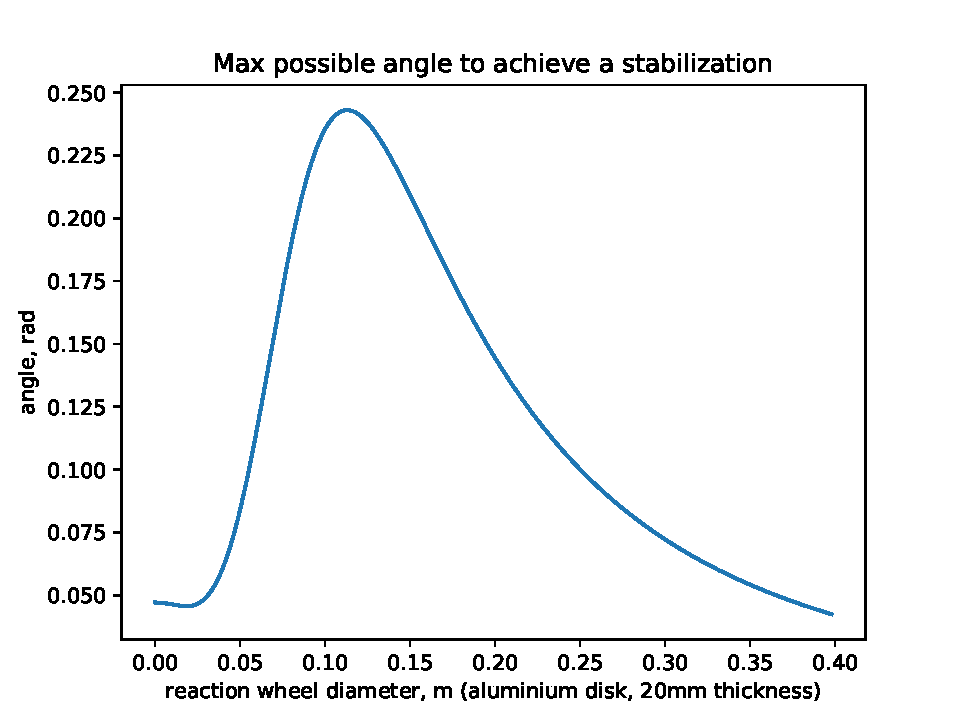
\includegraphics[width=.6\linewidth]{img/pendulum_dynamics}}
\caption{Самый выгодный диаметр маховика - 11см, при этом можно будет отклонить маятник на 0.24 радиана.}
\label{fig:rwdiameter}
\end{figure}
%Получается, что чем меньше маховик, тем легче стабилизировать (меньше массы поднимать), при этом быстрый подъём противо-ЭДС никого не волнует, системе выгоднее дать короткий, но сильный импульс. В таких условиях мне кажется наиболее разумным выбор маховика диаметром эдак сантиметров 10 (это уже полкило, если что).

\iffalse

\newpage
\section{Давайте разбираться с моментами}
Силы тяжести нет, трения нет, все моменты инерции равны единице.
$$
q_v = q_p + \theta
$$

\subsection{Неподвижный репер}

Возьмём в качестве обобщённых координат $\theta$ и $q_v$. Тогда лагранжиан запишется так:
$$
\mathcal{L} = \frac{1}{2} \dot \theta^2 + \frac{1}{2}\dot q^2_v
$$

Для удобства выпишем все частные производные:
\begin{align*}
\frac{\partial\mathcal L}{\partial\dot q_v} &= \dot q_v   && \frac{\partial\mathcal L}{\partial q_v} = 0\\
\frac{\partial\mathcal L}{\partial\dot\theta} &= \dot\theta && \frac{\partial\mathcal L}{\partial\theta} = 0\\
\end{align*}

Выпишем уравнения Лагранжа:

\begin{align*}
\frac{d}{dt}\left(\frac{\partial\mathcal L}{\partial\dot q_v}\right) - \frac{\partial\mathcal L}{\partial q_v} = \ddot q_v = \tau\\
\frac{d}{dt}\left(\frac{\partial\mathcal L}{\partial\dot \theta}\right) - \frac{\partial\mathcal L}{\partial \theta} = \ddot\theta = -\tau\\
\end{align*}

\subsection{Вращающийся репер}

Возьмём в качестве обобщённых координат $\theta$ и $q_p$. Тогда лагранжиан запишется так:
$$
\mathcal{L} = \frac{1}{2} \dot \theta^2 + \frac{1}{2}(\dot q_p+\dot\theta)^2
$$

Для удобства выпишем все частные производные:
\begin{align*}
\frac{\partial\mathcal L}{\partial\dot q_p} &= \dot q_p + \dot\theta && \frac{\partial\mathcal L}{\partial q_p} = 0\\
\frac{\partial\mathcal L}{\partial\dot\theta} &= 2\dot\theta +\dot q_p &&  \frac{\partial\mathcal L}{\partial\theta} = 0\\
\end{align*}

Выпишем уравнения Лагранжа. Предположим, что я не знаю действующих моментов, обозначу их через $x$ и $y$, буду их искать так, чтобы уравнения совпали с уравнениями из предыдущего параграфа.

\begin{align*}
\frac{d}{dt}\left(\frac{\partial\mathcal L}{\partial\dot q_p}\right) - \frac{\partial\mathcal L}{\partial q_p}= \ddot q_p + \ddot\theta = x\\
\frac{d}{dt}\left(\frac{\partial\mathcal L}{\partial\dot \theta}\right) - \frac{\partial\mathcal L}{\partial \theta}= 2\ddot\theta +  \ddot q_p   = y\\
\end{align*}

Перепишем наши уравнения движения следующим образом:

\begin{align*}
\ddot q_p = 2x - y\\
\ddot\theta = y - x
\end{align*}

Очевидно, что если $\ddot q_v = \tau$, то $\ddot q_p = 2\tau$, поскольку $q_v = q_p + \theta$, а $\ddot\theta = -\tau$. Запишем уравнения для $x$ и $y$:

\begin{align*}
\ddot q_p = 2x - y = 2\tau\\
\ddot\theta = y - x = -\tau
\end{align*}

Решением является $x=\tau, y=0$. ЧТД.

\fi

\end{document}
